\documentclass[conference, twocolumn]{IEEEtran}
% \setlength{\parskip}{1em}

\usepackage{amssymb,latexsym,amsmath,amsthm}

\usepackage{graphicx}
\graphicspath{ {./images/} }

\usepackage{xcolor}
\usepackage{subfig}
\usepackage{fancyvrb}
\usepackage{hyperref}

\newcommand{\Z}{\mathbb{Z}}
\newcommand{\set}[1]{\{\,#1\,\}}

%%%%%%%%%%%%%%%%%%%%%%%%%%%%%%
% Theorem/Proof Environments %
%%%%%%%%%%%%%%%%%%%%%%%%%%%%%%
\theoremstyle{plain}
\newtheorem{theorem}{Theorem}[section]
\newtheorem{lemma}[theorem]{Lemma}

\theoremstyle{definition}
\newtheorem{definition}[theorem]{Definition}

\theoremstyle{remark}
\newtheorem*{remark}{Remark}
\newtheorem*{remarks}{Remarks}
\newtheorem{exercise}{Exercise}

\begin{document}

\title{Demonstração analítica e numérica de propriedades dos grafos de Erdos Renyi e Watts Strogatz}

\author{
\IEEEauthorblockN{Regina Duarte}
\IEEEauthorblockA{\textit{Mestrado em Engenharia e Ciência de Dados} \\
\textit{Instituto Superior Técnico}\\
96986}
\and
\IEEEauthorblockN{Pedro Rio}
\IEEEauthorblockA{\textit{Mestrado em Engenharia e Ciência de Dados} \\
\textit{Instituto Superior Técnico}\\
97241}
}

\twocolumn[
  \begin{@twocolumnfalse}
    \maketitle
    \begin{abstract}
    Neste projeto analisamos algumas propriedades de dois tipos de grafos estudados em aula - o modelo de Erdos Renyi e o modelo de Watts Strogatz. Em  ambos os casos analisamos analiticamente e numericamente\cite{4} a distribuição do grau, o coeficiente de agrupamento e o percurso médio dos grafos, tal como como cada grafo se compara com grafos reais.
    \end{abstract}
  \end{@twocolumnfalse}
  \bigskip
]

\section{Grafo Erdos Renyi}
O grafo Erdos Renyi é um grafo aleatório com dois parametros, $n_{nodos}$ e $p_{ligação}$, onde $n_{nodos}$ é o número de nodos do grafo e $p_{ligação}$ é a probabilidade de um nodo $n_i$ estar ligado ao nodo $n_j$ para todo o $i$ e $j$. Aqui vamos considerar sempre que $n_{nodos}$ é suficientemente grande e que o grau médio de cada nodo é $<k>=np$.\cite{1}

\subsection{Distribuição do grau de um nodo}
Nesta secção vamos mostrar que no modelo Erdos Renyi, a distribuição de probabilidades do grau de cada nodo segue uma distribuição binomial de parametros $n_{nodos}-1$ e $p_{ligação}$ e que quando $n_{nodos}$ toma valores muito grandes a distribuição pode ser aproximada ao modelo poisson com parâmetro $(n_{nodos}-1) p_{ligação}$.

Sabemos que a probabilidade de um nodo $i$ se ligar a outro é dada por $p_{ligação}$. Assim cada nodo pode ligar-se aos outros $n_{nodos}-1$ com probabilidade $p_{ligação}$. Ou seja trata-se  de uma sucessão de acontecimentos onde o nodo $i$ se liga a outro nodo com probabilidade $p_{ligação}$ ou não se liga com probabilidade $1-p_{ligação}$.
Assim a probabilidade de um nodo $i$ ter grau $k$, i.e. ligar-se a $k$ nodos é dada por:

\begin{center}
$\binom{n_{nodos}-1}{k}p_{ligação}^{k}{(1-p_{ligação})}^{n_{nodos}-1-k}$
\end{center}

onde $p_{ligação}^{k}$ representa a probabilidade do nodo se ligar a $k$ nodos, multiplicado pela probabilidade do nodo $i$ não se ligar aos outros $n_{nodos}-1-k$ nodos e ainda multiplicado por todas as combinações possíveis dos nodos que se ligam ao nodo $i$, ${(1-p_{ligação})}^{n_{nodos}-1-k}$.
Ou seja, chegamos à conclusão que a distribuição do grau do grafo Erdos Renyi é binomial com parâmetros $n_{nodos}-1$ e $p_{ligação}$.

\begin{figure}[h]
    \centering
    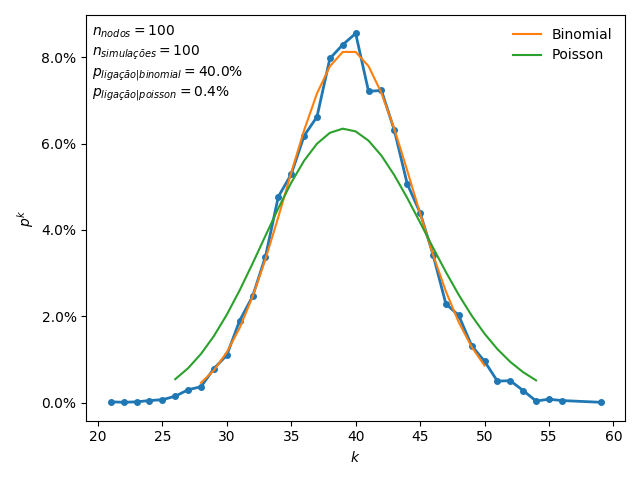
\includegraphics[width=1\linewidth]{images/erdos_renyi_degree_binomial_and_poisson_distributions_low_number_of_initial_nodes.png}
    \caption{\small Distribuição média de 100 simulações do grau do grafo de Erdos Renyi com $n_{nodos}=100$ e $p_{ligação}=40\%$}
    \label{fig:erdos_renyi_degree_binomial_and_poisson_distributions_low_number_of_initial_nodes}
\end{figure}

Na figura \ref{fig:erdos_renyi_degree_binomial_and_poisson_distributions_low_number_of_initial_nodes} simulámos 100 grafos de Erdos Renyi com $n_{nodos}=100$ e $p_{ligação}=40\%$ e confirmámos numericamente que a média da distribuição do grau de um nodo segue uma distribuição binomial com parâmetros $n_{nodos}-1$ e $p_{ligação}$.

Sendo $<k>$ o grau médio do grafo, sabemos que:
\begin{center}
$<k>=(n_{nodos}-1)p_{ligação} \Leftrightarrow p=\frac{<k>}{n_{nodos}-1}$.
\end{center}

Substituindo no limite ficamos com:

\begin{center}
$\lim_{n\rightarrow \infty} \frac{(n-1)!}{(n-1-k)!k!}{\frac{<k>}{n-1}}^{k}{(1-\frac{<k>}{n-1})}^{n-1-k} =$\\
$= \frac{<k>^k}{k!} \lim_{n\rightarrow \infty} \frac{(n-1)...(n-k)(n-1-k)...(1)}{(n-1-k)!}
\\ \times \frac{1}{(n-1)^k}
{(1-\frac{<k>}{n-1})}^{n-1}{(1-\frac{<k>}{n-1})}^{-k} = $\\

 $=  \frac{<k>^k}{k!} \lim_{n\rightarrow \infty} \frac{(n-1)...(n-k)}{(n-1)^k} {(1-\frac{<k>}{n-1})}^{n-1}{(1-\frac{<k>}{n-1})}^{-k} =$\\

$=  \frac{<k>^k}{k!} \lim_{n\rightarrow \infty} \frac{(n-1)}{(n-1)}{...}\frac{(n-k)}{(n-1)}{(1-\frac{<k>}{n-1})}^{n-1}{(1-\frac{<k>}{n-1})}^{-k} $\\
\end{center}

Temos que:
\begin{center}
$ \lim_{n\rightarrow \infty} \frac{(n-1)}{(n-1)} {...}\frac{(n-k)}{(n-1)} \rightarrow 1$, \\
$\lim_{n\rightarrow \infty}{(1-\frac{<k>}{n-1})}^{n-1} \rightarrow 1$
\end{center}

e que
\begin{center}

$ \lim_{n\rightarrow \infty}{(1-\frac{<k>}{n-1})}^{-k} \rightarrow e^{-<k>}$\\
\end{center}

logo,\\

\begin{left}
$ \lim_{n\rightarrow \infty} \frac{(n-1)}{(n-1)}{...}\frac{(n-k)}{(n-1)}{(1-\frac{<k>}{n-1})}^{n-1}{(1-\frac{<k>}{n-1})}^{-k} \rightarrow$ $\rightarrow e^{-<k>}$
\\
\end{left}

Assim,\\

\begin{center}
$\lim_{n\rightarrow \infty} \binom{n-1}{k}p^{k}{(1-p)}^{n-1-k} \rightarrow \frac{<k>^k}{k!}e^{-<k>}$
\end{center}

e concluímos que quando o número de nodos do grafo é muito grande podemos aproximar a distribuição do grau pela poisson com o parametro igual ao grau médio do grafo.

\begin{figure}[h]
    \centering
    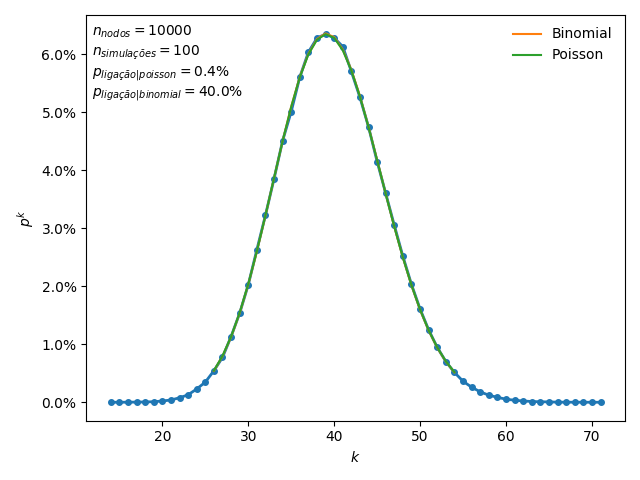
\includegraphics[width=1\linewidth]{images/erdos_renyi_degree_binomial_and_poisson_distributions_high_number_of_initial_nodes.png}
    \caption{\small Distribuição média de 100 simulações do grau do grafo de Erdos Renyi com $n = 10000$ e $p = 40\%$}
    \label{fig:erdos_renyi_degree_binomial_and_poisson_distributions_high_number_of_initial_nodes}
\end{figure}

Na figura \ref{fig:erdos_renyi_degree_binomial_and_poisson_distributions_high_number_of_initial_nodes} repetimos as simulações da figura \ref{fig:erdos_renyi_degree_binomial_and_poisson_distributions_low_number_of_initial_nodes}, aumentando o número de nodos para 10000 e alterando a probabilidade de um nodo se ligar a outro de modo a manter o grau médio das simulações da figura \ref{fig:erdos_renyi_degree_binomial_and_poisson_distributions_low_number_of_initial_nodes}, tendo em conta que a média da distribuição binomial é $(n - 1) p$.

Confirmamos assim que quando $n$ é muito grande a distribuição média do grau de um nodo do grafo de Erdos Renyi segue uma distribuição de poisson com parêmetro $<k>$.

\subsection{Coeficiente de agrupamento}
Vamos falar agora do coeficiente de agrupamento do modelo ER.
Para começar sabemos que o coeficiente de agrupamento de um nodo é dado por:
\begin{center}
$Ci = \frac{numero\ de\ links\ entre\ os\ vizinhos\ de\ i}{total\ de\ links\ entre\ os\ vizinhos}$
\end{center}
Logo o coeficiente de agrupamento médio do grafo é dado por $C= \frac{\sum{i=1}^{n} Ci}{n}$\\
Vamos supor que o grau de um nodo $i$ é igual a $k_i$. Ou seja temos $k_i$ nodos vizinhos de $i$. Assim, o número de links possíveis entre os vizinhos de i é dado por $\binom{k_i}{2} = \frac{k_i(k_i-1)}{2}$\\

Como os links são formados com probabilidade $p$, sabemos que o numero de links entre os vizinhos de $i$ vai ser em média $\frac{k_i(k_i-1)}{2}p$\\

Logo,\\
\begin{center}
$Ci = \frac{\frac{k_i(k_i-1)}{2}p}{\frac{k_i(k_i-1)}{2}} = p = \frac{<k>}{n-1}$, logo $C=\frac{\sum_{i=1}^{n} p}{n} = \frac{np}{n} = Ci$
\end{center}

Concluimos, então, que no modelo de Erdos Renyi o coeficiente de agrupamento diminui quando $n$ aumenta, o que implica que quanto maior o número de nodos do grafo, menor o coeficiente de agrupamento. Na prática a maior parte dos grafos de Erdos Renyi vão ter um coeficiente de agrupamento muito baixo, o que não se verifica na grande maioria dos grafos reais.

\subsection{Comprimento do percurso médio}
Na secção anterior vimos que o coeficiente de agrupamento é muito pequeno se considerarmos $n$ grande. Para calcularmos analiticamente o comprimento do percurso médio destes grafos vamos usar esse resultado. Consideremos $n$ suficientemente grande tal que podemos aproximar o coeficiente de agrupamento a zero. Assim, o grafo vai ter uma estrutura de árvore.Se considerarmos que cada nodo tem em média grau $<k>$ podemos dizer que cada nodo $i$

\begin{itemize}
    \item à distância $1$ tem $<k>$ vizinhos;
    ...
    \item à distância $m$ tem $<k>^m$ vizinhos.
\end{itemize}

Assim se quisermos saber o número de vizinhos de um nodo até à distância $j$ temos de somar todos os nodos vizinhos da distancia $1$ ate à distancia $j$
Logo o número de nodos até à distancia $j$, $N(j)$ é dado por:\\

$\sum_{i=1}^{j} <k>^i$ \\

Como se trata de uma serie geometrica temos que\\

$N(j)= \frac{<k>^{j+1}-1}{<k>-1}$\\

Sabemos que à distancia máxima o número de vizinhos do nodo $i$ corresponde ao numero total de nodos $n$. Logo $N(d_{max})=n$\\

Assim, temos que \\
\begin{center}
$n = \frac{<k>^{dmax+1}-1}{<k>-1}$\\
${}$\\
$n \approx \frac{<k>^{dmax+1}}{<k>} \approx <k>^{dmax}$\\
${}$\\
$d_{max} \approx \frac{\log n}{\log <k>}$
\end{center}

Concluimos então que a distância máxima entre dois nodos é dado pela expressão acima e que o comprimento do percurso médio pode ser aproximado por esse valor.\\

\begin{figure}[h]
    \centering
    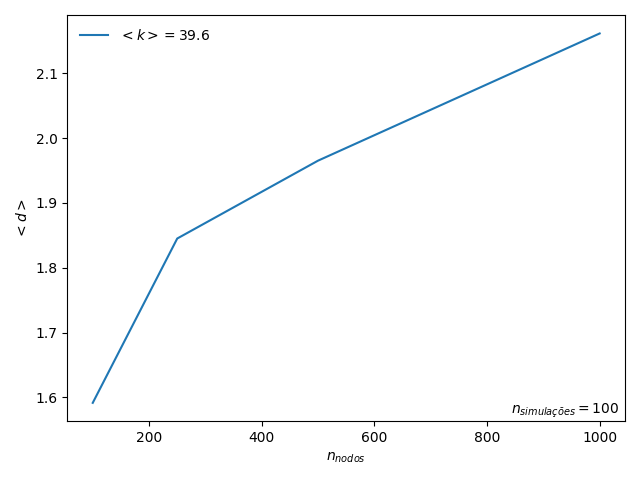
\includegraphics[width=1\linewidth]{images/erdos_renyi_average_path_length.png}
    \caption{\small Média das distâncias médias entre dois nodos em 100 grafos de Erdos  Renyi, para $<k> = 39.6$, consoante o número de nodos.}
    \label{fig:erdos_renyi_average_path_length}
\end{figure}

Na figura \ref{fig:erdos_renyi_average_path_length} simulámos para vários $n_{nodos}$, 100 grafos de Erdos Renyi, alterando os valores de $p_{ligação}$ de modo a manter $<k> = 39.6$ e calculando a média das distâncias médias entre os nodos cada grafo. Verificámos que o comprimento do percurso médio adopta $<d> \approx \frac{\log n}{\log <k>}$, o que é consistente com os efeitos do mundo pequeno de grafos reais em que o comprimento do percurso médio aumenta de forma logarítmica e não linear.

\section{ Grafo Watts e Strogatz}
Neste modelo o grafo é construido da seguinte forma: os nodos são dispostos numa forma circular e cada nodo está ligado aos seus $2k$ vizinhos mais proximos, ie, o nodo está ligados aos $k$ vizinhos mais proximos à esquerda e $k$ vizinhos mais proximos à direita.
Posteriormente temos um parametro $p$ que corresponde à probabilidade de reordenar cada link que está ligado a cada nodo $i$ e aos seus vizinhos da esquerda, sendo que cada link destes só pode ser reordenado uma vez e na reordenação tem obrigatoriamente de ficar ligado ao nodo $i$, podendo só mudar de vizinho.
Depois da reordenação ficamos uma instância do grafo de Watts Strogatz\cite{2}, que apresenta algumas propriedades mais consistentes com grafos reais.

\subsection{Distribuição do grau}
Começamos por notar que quando $p=0$, ou seja, quando o grafo mantem as suas condições iniciais, o grau de todos os nodos é igual a $2k$. Para $p>0$ denotamos por $P_{p}(c)$ a probabilidade do grau de um nodo ser $c$ dado que a probabilidade de reodenação dos link é $p$.

Como só os link que estão associados aos vizinhos da esquerda é que podem ser reordenados e a reordenação mantém o link associado ao nodo inicial, o número de links mínimo de cada nodo $i$ é igual a $k$. Assim, podemos dizer que cada nodo $i$ vai ter grau $c_{i}=k+n_{i}$ onde $n_{i}$ corresponde à soma dos links onde $i$ era vizinho à esquerda mas que não foram reordenados com probabilidade $1-p$, $n_{i}^{1}$, com os links que foram reordenados e passaram a estar associados a $i$ com probabilidade $\frac{p}{n}$, $n_{i}^{2}$ pois a reordenção é aleatória entre todos os nodos.\\

Assim, a distribuição de $n_{i}^{1}$ vai ser uma binomial $(k,1-p)$ pois cada link à direita do nodo $i$ não é reordenado com probabilidade (1-p) e são $k$ links nestas condições, que vão ser ou não reordenados (pois o nodo $i$ tem $k$ vizinhos à direita). $n_{i}^{2}$  também vai ter uma distrbuição binomial com parametros $(nk, p/n)$ pois existem $kn$ links que podem ser reassociados ao nodo $i$ (os k links de todos os nodos do grafo) com probabilidade $\frac{p}{n}$, para $n$ grande esta distribuição pode ser aproximada a uma distribuição poisson com parâmetro $nk\times{\frac{p}{n}}= kp$.\\

Logo temos que,\\
\begin{center}
    $P_{p}(n_{i}^{1})= \binom{k}{n_{i}^{1}} (1-p)^{n_{i}^{1}} p^{k-n_{i}^{1}}$
\end{center}
e que \\
\begin{center}
    $P_{p}(n_{i}^{2}) = \frac{(kp)^{n_{i}^{2}}}{n_{i}^{2}!} e^{-kp}$
\end{center}
Como $n_{i}=n_{i}^{1}+n_{i}^{2}$ e não sabemos exatamente a quantidade exata de cada um, $P_{p}(c)$ vai ser igual ao somatório das probabilidades de todas as possibilidades de $n_{i}^{1}$ e $n_{i}^{2}$\\

Logo temos que\\
\begin{center}
    $P_{p}(c)= \sum_{n=0}^{min(c-k,k)} \binom{k}{n}(1-p)^{n} p^{k-n} \times \frac{(kp)^{c-k-n}}{(c-k-n)!} e^{-kp}$
\end{center}
onde $n=n_{i}^{1}$ e $c-k-n=n_{i}^{2}$.

\begin{figure}[h]
    \centering
    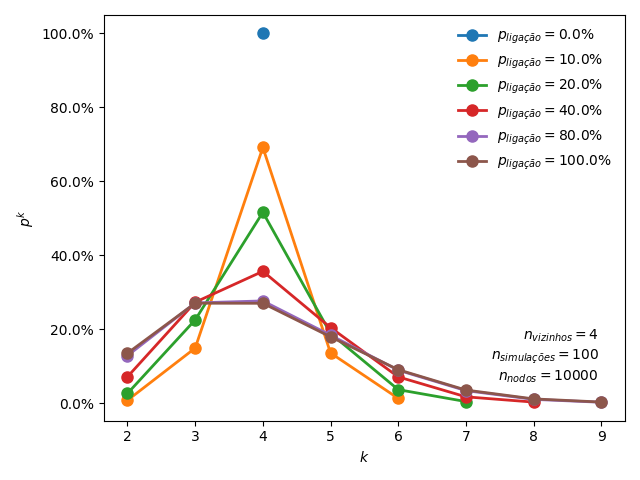
\includegraphics[width=1\linewidth]{images/watts_strogatz_degree_distribution.png}
    \caption{\small Distribuições médias de 100 simulações do grau do grafo de Watts Strogatz com $n = 10000$ para vários $p$.}
    \label{fig:watts_strogatz_degree_distribution}
\end{figure}

Na figura \ref{fig:watts_strogatz_degree_distribution} confirmámos numericamente que para $p = 0\%$ a média das distribuições do grau médio é $2k$ e que à medida que $p$ se aproxima de 100\% a média das distribuições do grau médio se aproxima de uma binomial com média $2k - 1$. Para chegar a esta conclusão foram simulados 100 grafos de Watts Strogatz com 10000 nodos e várias probabilidades de um nodo se ligar a outro de modo a manter a média do grau constante.

\subsection{Coeficiente de agrupamento}
Como já vimos no modelo anterior o coeficiente de agrupamento de cada nodo $i$ é dado por:\\
\begin{center}
    $Ci = \frac{numero\ de\ links\ entre\ os\ vizinhos\ de\ i}{total\ de\ links\ entre\ os\ vizinhos}$
\end{center}
Vamos tentar perceber qual é o coeficente de agrupamento de um grafo onde $p=0$.\\
Aqui, todos os nodos têm grau igual a $2k$, logo o número máximo de links possíveis entre os vizinhos é dado por $\binom{2k}{2} = \frac{2k(2k-1)}{2}$.Como $p=0$, o número de links entre os vizinhos de cada nodo também é constante e é dado por $\frac{3k(k+1)}{2}$\\
Assim, o coeficiente de agrupamento para $p=0, C(0)$ é dado por:

\begin{center}
    $C(0) = \frac{\frac{3k(k+1)}{2}}{\frac{2k(2k-1)}{2}}=\frac{3k(k-1)}{2k(2k-1)}$
\end{center}

Sabemos que a probabilidade de um link ser reordenado é $p$, logo a probabilidade de dois vizinhos de um nodo $i$ permanecerem conectados depois da reordenação é dado por $1-p$. Esta é também a probabilidade de cada um desses vizinhos continuar conectado ao nodo $i$. Assim a probabilidade do triângulo formado inicialmente entre o nodo $i$ e dois dos seus vizinhos permanecer depois da reordenação é $(1-p)^3$.\\ Logo, em média, o número de links entre os vizinhos do nodo $i$  é igual ao numero inicial de links entre os vizinhos multiplicado por $(1-p)^{3}$ ou seja $\frac{3k(k+1)}{2}\cdot (1-p)^{3}$. Deste modo, podemos aproximar o coeficiente de agrupamento de um nodo, pela média do coeficiente de agrupamento obtendo que $C_{i}(p)= C(O)\times (1-p)^{3}$.

Assim verificamos que quando $p<1$ o agrupamento de um nodo no grafo de Watts Strogatz é superior ao de um nodo no grafo de Erdos Renyi, tal como acontece em grafos reais.\cite{3} Também observamos nas simulações que apresentamos na figura \ref{fig:watts_strogatz_clustering_coefficient_and_average_path_length} que é necessária muita aleatoriedade para destruir agrupamentos.

\begin{figure}[h]
    \centering
    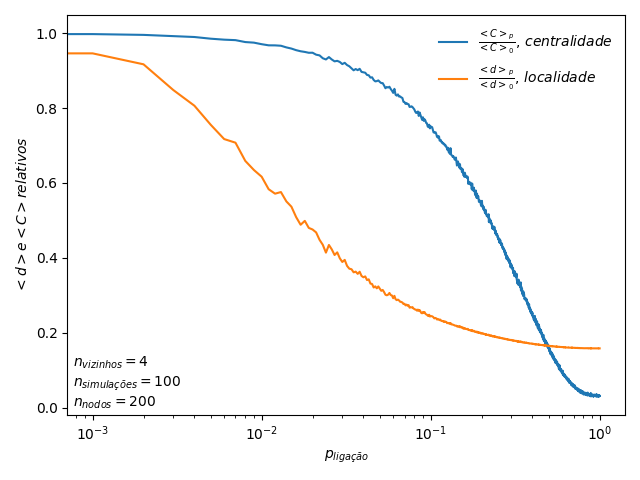
\includegraphics[width=1\linewidth]{images/watts_strogatz_clustering_coefficient_and_average_path_length.png}
    \caption{\small Agrupamentos e comprimento do percurso médio relativos de 20 simulações do grau do grafo de Watts Strogatz com $n = 10000$ para vários $p$.}
    \label{fig:watts_strogatz_clustering_coefficient_and_average_path_length}
\end{figure}

\subsection{Comprimento do percurso médio}
Nesta última secção vamos analisar o comprimento do percurso médio do grafo de Watts Strogatz quado $p=0$. Para quando $p>0$ a analise pode ser vista em \cite{2}.
Como o grafo é circular e os links não se alteraram, todos os nodos têm grau $2k$. Assim, o comprimento máximo entre dois nodos vai ser o comprimento entre os nodos que estão nos extremos de uma semi-circunferência do grafo.
Se $k=1$, os nodos estavam ligados apenas aos nodos do seu lado esquerdo e direito e portanto o caminho mais curto entre os extremos da semi-circumferência seria $\frac{n}{2}$. Assim, para qualquer $k$ temos que o caminho mais curto entre os nodos mais distantes é $\frac{n}{2k}$
Como este grafo é um grafo simétrico e circular é fácil notar que o comprimento do percurso médio vai ser dado então por aproximadamente $\frac{n}{4k}$.

Calculámos a distância média entre dois nodos nas simulações que apresentamos na figura \ref{fig:watts_strogatz_clustering_coefficient_and_average_path_length} e verificámos que pouca aleatoriedade consegue destruir a localidade dos grafos.

\bibliographystyle{plain}
\bibliography{bib}

\end{document}